% !TeX root = main.tex

% ============================================================
% thesis-sync entry: 2026-07-06_coupled-bodytail-actuator-design
% Type: design decision + numeric data
% Insertable section block (no preamble). Requires: graphicx.
% Figure \includegraphics lines are COMMENTED so the file compiles standalone.
% ============================================================

\section{COUPLED BODY--TAIL ACTUATOR}
\label{sec:lizard-bodytail}

\subsection{Segment Geometry}

Each of the body and tail segments is a miniaturized fiber-reinforced
cylindrical actuator with a tri-axial chamber cross-section, geometrically
identical to the omnidirectional bending actuator of
Section~\ref{sec:inchworm-actuator}, scaled down by a factor of three. The
silicone body is a cylinder of 6~mm outer diameter and 26~mm length
(33~mm overall actuator length including end interfaces), whose interior
is divided by internal walls converging at the central axis into three
radially symmetric chambers of 120$^{\circ}$ each
\cite{Yan2016ThreeChamber,Moutousi2024Omnidirectional}. The outer wall
thickness is 0.4~mm. Selective pressurization of one chamber, or
concurrent pressurization of two chambers, produces bending in the
corresponding direction, so that the segment bends omnidirectionally in
space; concurrent pressurization of all three chambers produces
elongation.

\subsection{Fiber Reinforcement}

Radial expansion of the pressurized chambers is constrained by
circumferential fiber reinforcement wound around the outer surface. In
contrast to the helical winding common in fiber-reinforced actuators, the
reinforcement consists of discrete parallel circumferential loops with an
average spacing of 1.5~mm. The loops are applied by hand after dipping
the fiber in uncured silicone; the excess silicone is removed
by scraping the fiber with tweezers, and the spacing value is therefore
an average subject to manufacturing variability. In addition to the
circumferential loops, a single inextensible fiber runs along the central
axis of the segment, through the junction of the three internal walls.
The central fiber constrains axial elongation of the neutral axis, so
that chamber inflation is converted preferentially into bending curvature
rather than stretch; its measured effect on the pressure--angle
characteristic is reported in Section~\ref{sec:lizard-characterization}.

\subsection{Coupled Configuration}

The body and tail segments are mounted collinearly on opposite faces of a
rigid central connector (Section~\ref{sec:lizard-connector}), which routes
their chambers pneumatically and carries the pressure inlet. The two
segments are geometrically identical; their functional asymmetry --- the
segment closer to the inlet exhibits larger quasi-static bending --- arises
from the pneumatic transmission path rather than from the segment
geometry. By convention, the segment closer to the inlet, i.e., the
segment exhibiting the larger bending amplitude, is designated as the
body, and the distal segment as the tail. This assignment prioritizes
wall-transition behavior, in which the anterior part of the robot must
lift and reorient, while the tail follows.

% --- Figures (paths to be fixed by the author; commented for compilation) ---
\begin{figure}[tb]
  \centering
  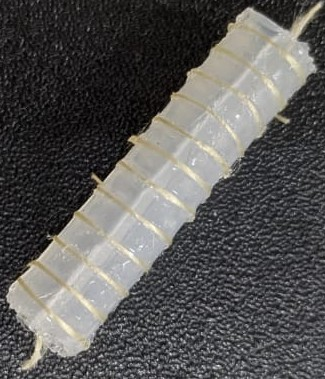
\includegraphics[height=38mm]{figures/centralfiberTopview.jpeg}
  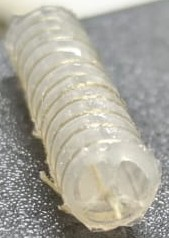
\includegraphics[height=38mm]{figures/centralfiberSideview.jpeg}
  \caption{Miniaturized three-chambered segment used for the body and
  tail. (a)~Axial view of the cast segment, showing the three
  120$^{\circ}$ chambers converging at the central axis. (b)~Side view of
  the segment with the parallel circumferential fiber loops at an average
  spacing of 1.5~mm.}
  \label{fig:lizard-segment}
\end{figure}

\begin{figure}[tb]
  \centering
  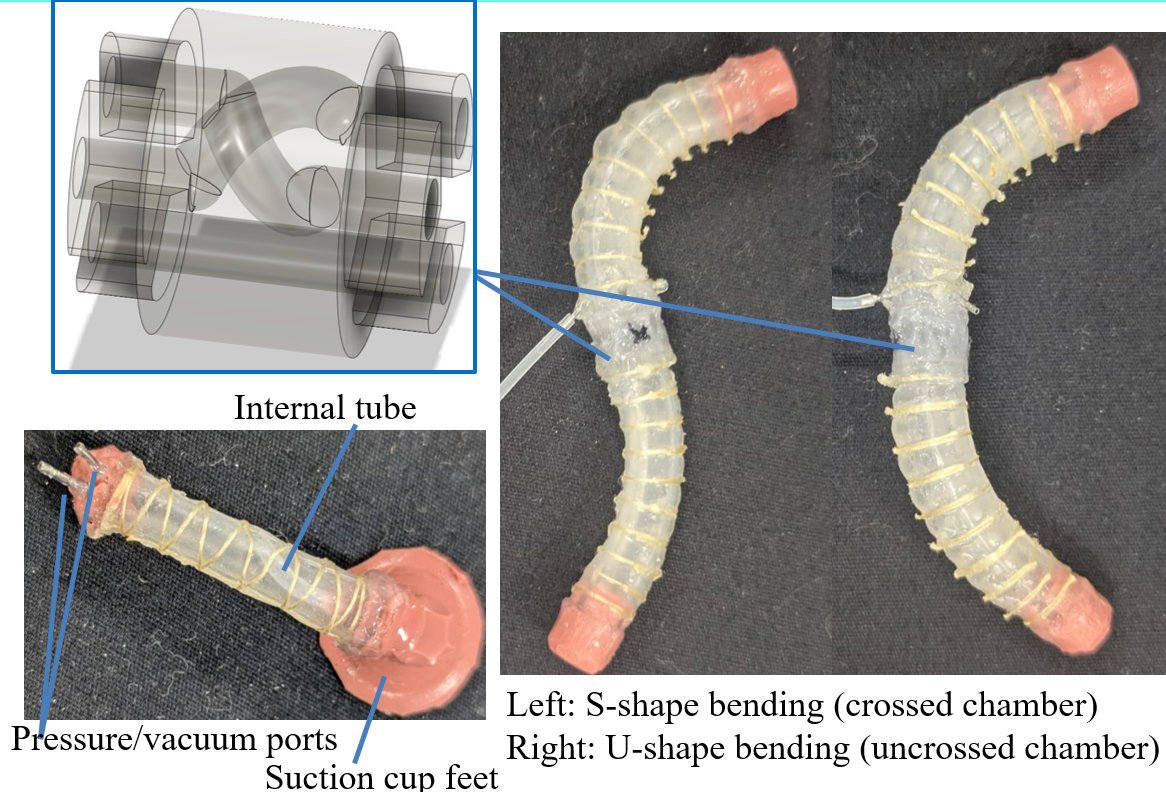
\includegraphics[width=0.95\columnwidth]{figures/lizard_actuators_details.png}
  \caption{Details of the actuator hardware. (a)~CAD view of the central
  connector with its internal channel routing. (b)~Leg actuator with the
  pressure and vacuum ports and the suction-cup foot indicated.
  (c)~S-shaped bending of the coupled body--tail unit obtained through the
  crossed chamber path. (d)~U-shaped bending obtained through the
  uncrossed chamber path.}
  \label{fig:lizard-actuator-details}
\end{figure}
